\chapter{Conclusions}\label{ch:7-conclusions}
The MicroBooNE experiment was designed to clarify the nature of a low-energy excess of electron-like events observed by the MiniBooNE experiment. 

We implemented an algorithm which employs the information coming from the optical system and the TPC of the MicroBooNE detector to select a sample enriched with $\nu_e$~CC0$\pi$-Np events. We show that it is possible to reject the cosmic and neutrino backgrounds by applying rectangular cuts on kinematic and calorimetric variables or by exploiting the classification power of the Boosted Decision Trees. In particular, we showed that the energy loss per length $dE/dx$ can be used to distinguish between electrons and photons interacting in a LArTPC. The selection was applied on a small sub-sample of the data collected by triggering on the Booster Neutrino Beam and validated on two orthogonal side-bands enriched with CC and NC $\nu_{\mu}$ interactions. The systematic uncertainties related to the cross-section, flux, and detector simulation were evaluated. The selection was also applied to an independent data sample acquired by triggering on the Neutrino at the Main Injector beam, measuring the significance of the presence of electron neutrinos in the beam. 
We measured the current significance to the low-energy excess with an expected exposure of the MicroBooNE detector of $13.2\times10^{20}$ protons-on-target. The performances needed to reach a $5\sigma$ sensitivity were measured.

\begin{figure}[htbp]
    \centering
    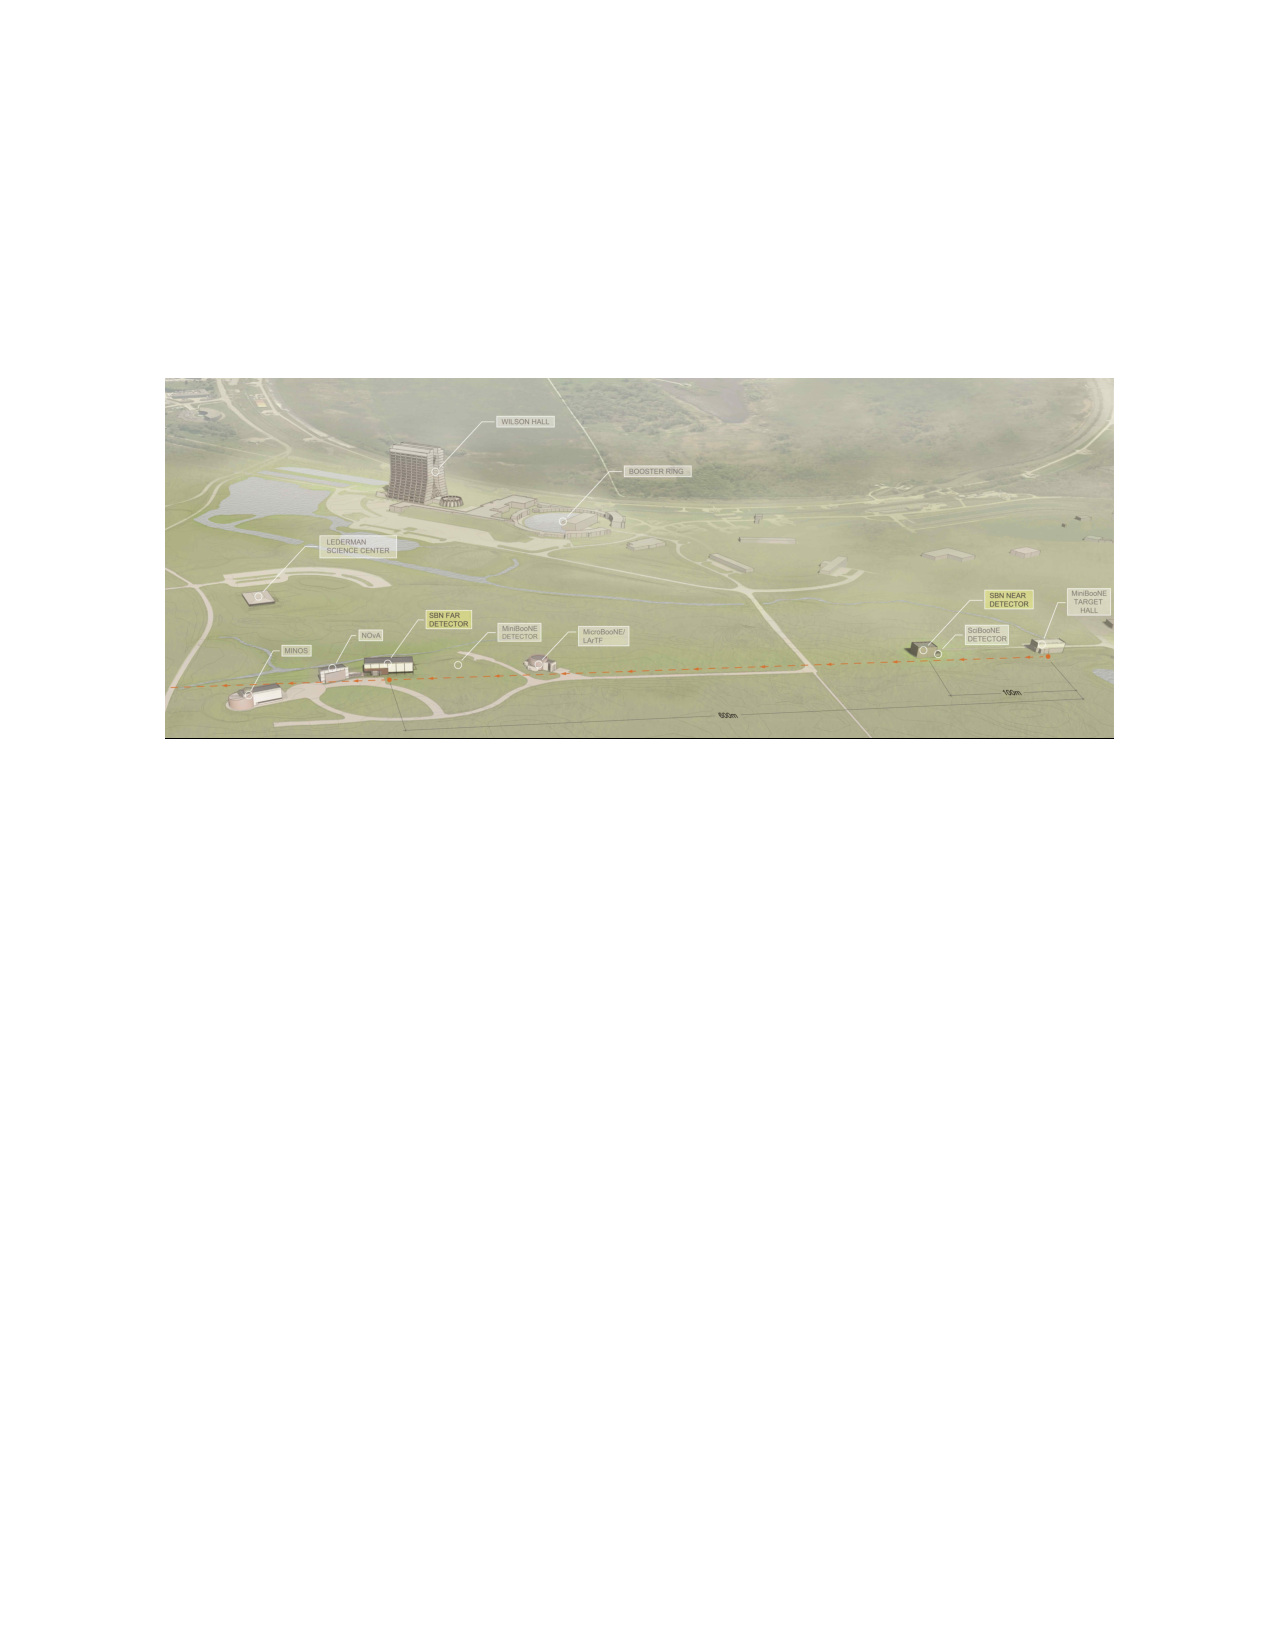
\includegraphics[width=0.9\linewidth]{figures/sbn_aerial.pdf}
    \caption{Aerial view of the Fermilab campus with the position of the three detectors forming the future Short Baseline Neutrino program. From \cite{Antonello:2015lea}.}
    \label{fig:sbn_aerial}
\end{figure}

MicroBooNE is the first step of the broader Short Baseline Neutrino (SBN) program at Fermilab \cite{Antonello:2015lea}. In this program, two other LArTPCs will be placed on-axis with the Booster Neutrino Beamline. The SBND detector (formerly known as LAr1-ND \cite{Adams:2013uaa}) will be placed close to the neutrino beam target and the refurbished ICARUS T600 detector \cite{Varanini:2017pvw} will be placed 600~m far from the target, 130~m farther than MicroBooNE (Figure \ref{fig:sbn_aerial}).

\begin{figure}[htbp]
    \centering
    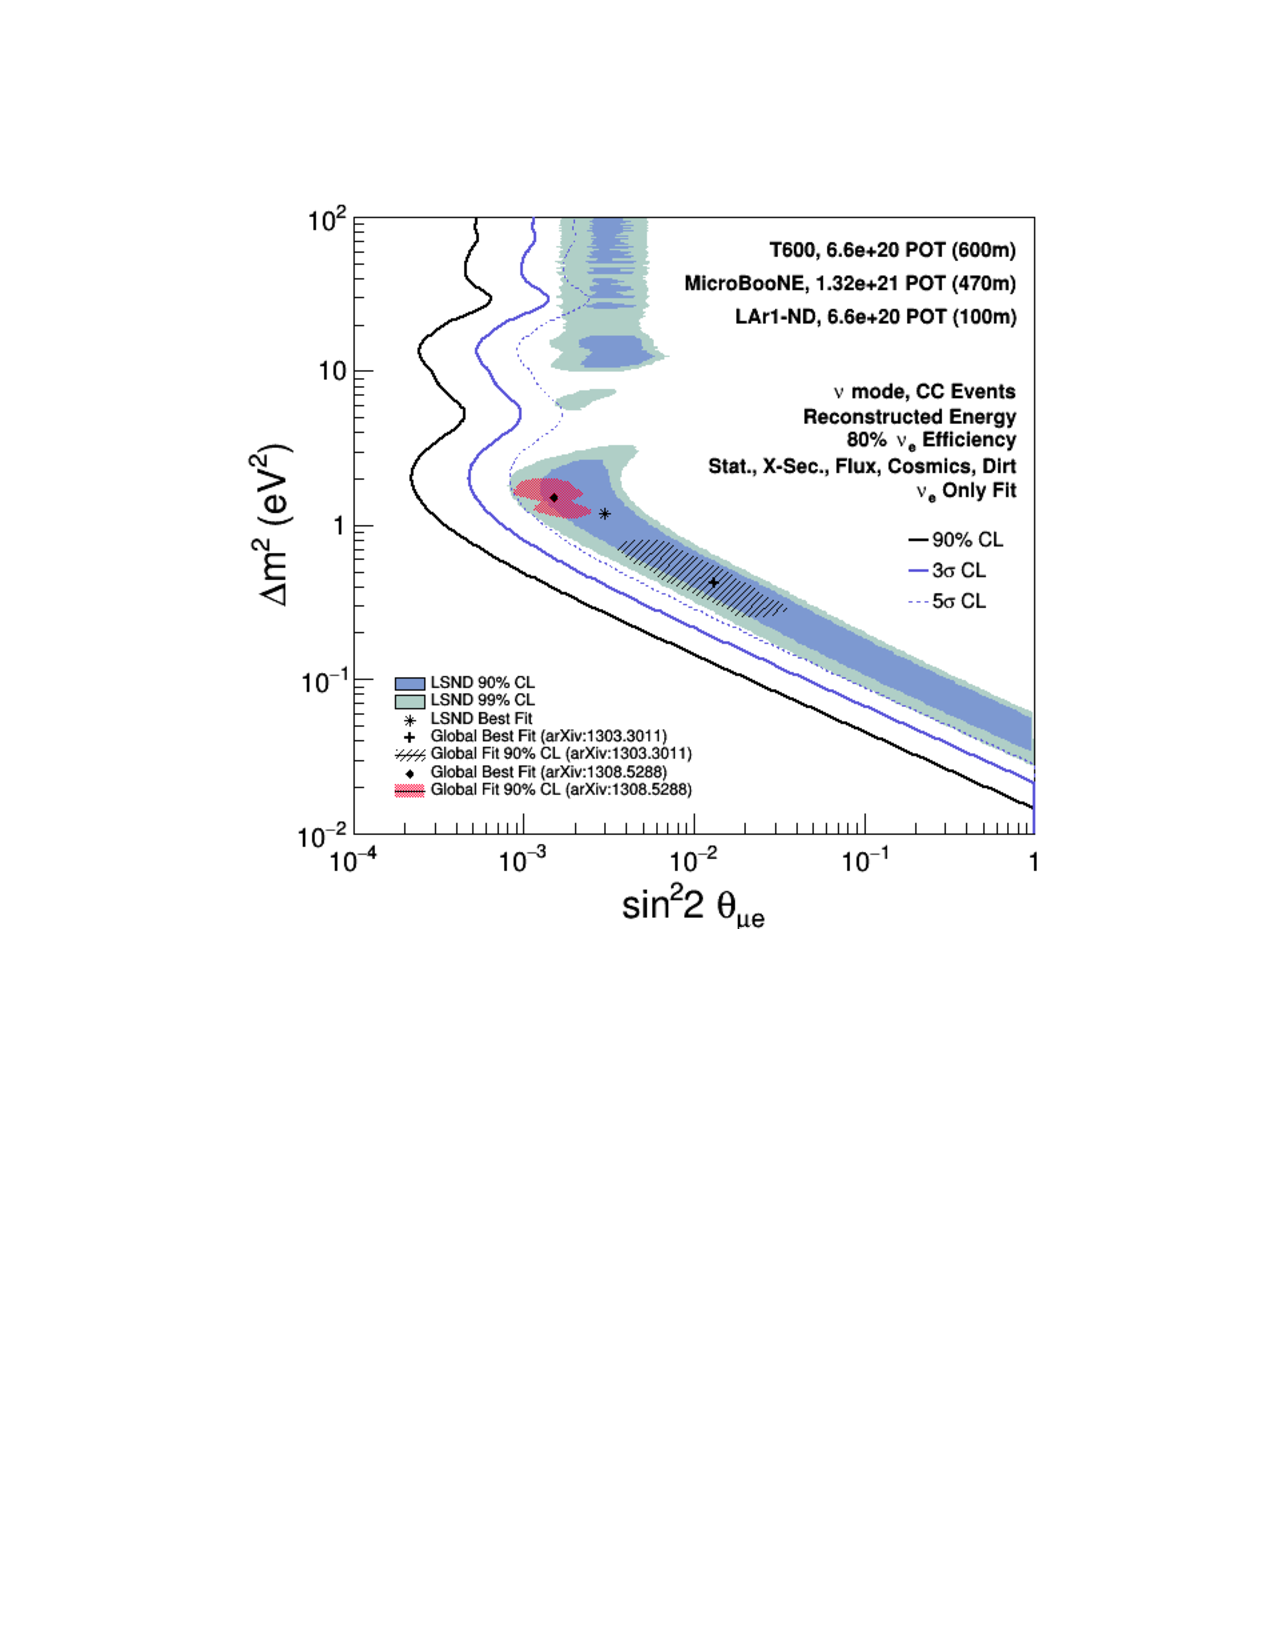
\includegraphics[width=0.75\linewidth]{figures/sbn_sensitivity.pdf}
    \caption{Sensitivity of the SBN Program to $\nu_{\mu}\rightarrow\nu_e$ oscillation signals. The filled areas correspond to the current allowed regions and the lines represent the sensitivity of the SBN program at different confidence levels. From \cite{Antonello:2015lea}.}
    \label{fig:sbn_sensitivity}
\end{figure}

The presence of three detectors on the same beamline employing the same technology will allow to constrain the cross-section, flux, and detector systematic uncertainties. The data coming from three detectors placed at different distances will allow to observe an eventual oscillation pattern and set the best limit on the search for sterile neutrino oscillations in the eV region. Figure \ref{fig:sbn_sensitivity} shows the sensitivity of the SBN program to $\nu_{\mu}\rightarrow\nu_e$ oscillations, assuming background rejection through topological cuts and with the aid of an external cosmic-ray tagger. 

